\documentclass{article}
\usepackage{tikz, comment}
\usepackage{pifont}
\usepackage{fontspec}
\usetikzlibrary{arrows, decorations.markings, decorations.pathreplacing}
\begin{comment}
:Title: Not defined yet
:Tags: average rate of change, arc ;area using parametric equations,parametric integral formula;approximation by differentials;area under a curve;root
:Prob: 0.4128;0.3789;0.3782;0.3624;0.3544
:Slug: No name yet

Description Here.........
\end{comment}
\begin{document}\centering

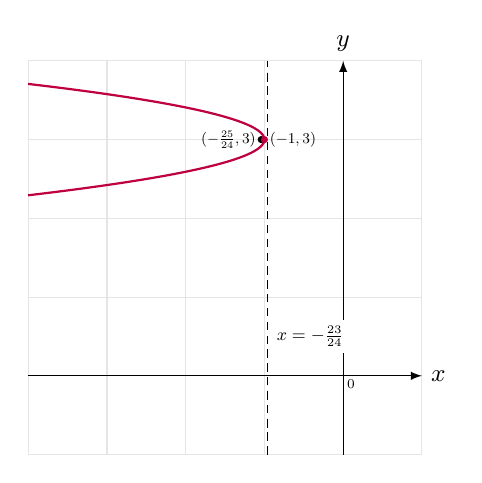
\begin{tikzpicture}[>=latex,xscale=.5*2, yscale=.5*2][font=\sf\small]

\draw[xstep=1cm,ystep=1cm,color=gray!20] (-4, -1) grid (1, 4);

\draw[->] (-4, 0) -- (1, 0)node[right] {\small $x$};
\draw[->] (0, -1) -- (0, 4)node[above] {\small $y$};

\clip[] (-4, -1) rectangle (1, 4);


\draw[purple, thick, samples=100, smooth, domain=-1.3+3:1.3+3, variable=\y]
plot ({-1-6*(\y-3)^2}, {\y});

\draw[fill] ({-25/24}, {3}) circle(0.075/2) node[black, left, xshift=0, yshift=0, scale=0.6] {$(-\frac{25}{24}, 3)$};

\draw[purple, fill] ({-1}, {3}) circle(0.075/2) node[black, right, xshift=0, yshift=0, scale=0.6] {$(-1, 3)$};

\draw[densely dashed, samples=100, smooth, domain=-1:4, variable=\y]
plot ({-23/24}, {\y});
\node[right, xshift=1, yshift=0, fill=white, scale=0.7] at ({-23/24},{0.5}) {$x=-\frac{23}{24}$};

\node[scale=0.7] at (0.2/2, -0.2/2) {\scriptsize$0$};

\end{tikzpicture}
\end{document}